\documentclass{../../templates/lkx_pset}

\title{Ling 105 Problem Set 7}
\author{Lev Kruglyak}
\due{November 8, 2024}

\usepackage{tipa}


\begin{document}
\maketitle
% # A tibble: 5 × 2
%   vowel avg_duration
%   <chr>        <dbl>
% 1 i             93.8
% 2 u             95.9
% 3 e            114. 
% 4 o            128. 
% 5 ae           128. 
% # A tibble: 2 × 2
%   vowel median_duration
%   <chr>           <dbl>
% [1] "The difference is significant."
% `geom_smooth()` using formula = 'y ~ x'
% `geom_smooth()` using formula = 'y ~ x'
% [1] "Number of words with two or more nasals in a row: 251"
% [1] "Number of words that both begin and end with a nasal: 3134"
% [1] "Percentage of time 't' is deleted in the word 'what': 64.6968534151957 %"
% > source("~/Documents/Harvard/Ling105/pset7/pset7.R")
%   mean_duration
% 1      93.76147
%   median_duration
% 1              81
% # A tibble: 5 × 2
%   vowel avg_duration
%   <chr>        <dbl>
% 1 i             93.8
% 2 u             95.9
% 3 e            114. 
% 4 o            128. 
% 5 ae           128. 
% # A tibble: 2 × 2
%   vowel median_duration
%   <chr>           <dbl>
% 1 e                85  
% 2 i                53.5
% [1] "W statistic: 30"
% [1] "p-value: 0.0161616161616162"
% [1] "The difference is significant."
% `geom_smooth()` using formula = 'y ~ x'
% `geom_smooth()` using formula = 'y ~ x'

\begin{problem}{1}
Load \texttt{vowels2.txt}. Make a density plot (\texttt{geom\_density}) of the duration of the vowel [i]. What is the mean and median duration of [i]? Judging by the plot, is the modal duration (approximate peak of the distribution) higher or lower than the median duration?
\end{problem}

The mean duration of [i] is $93.76$ ms and the median duration is $81$ ms. Based on the density plot, the modal duration is lower than the median duration because the distribution skews right.

\begin{center}
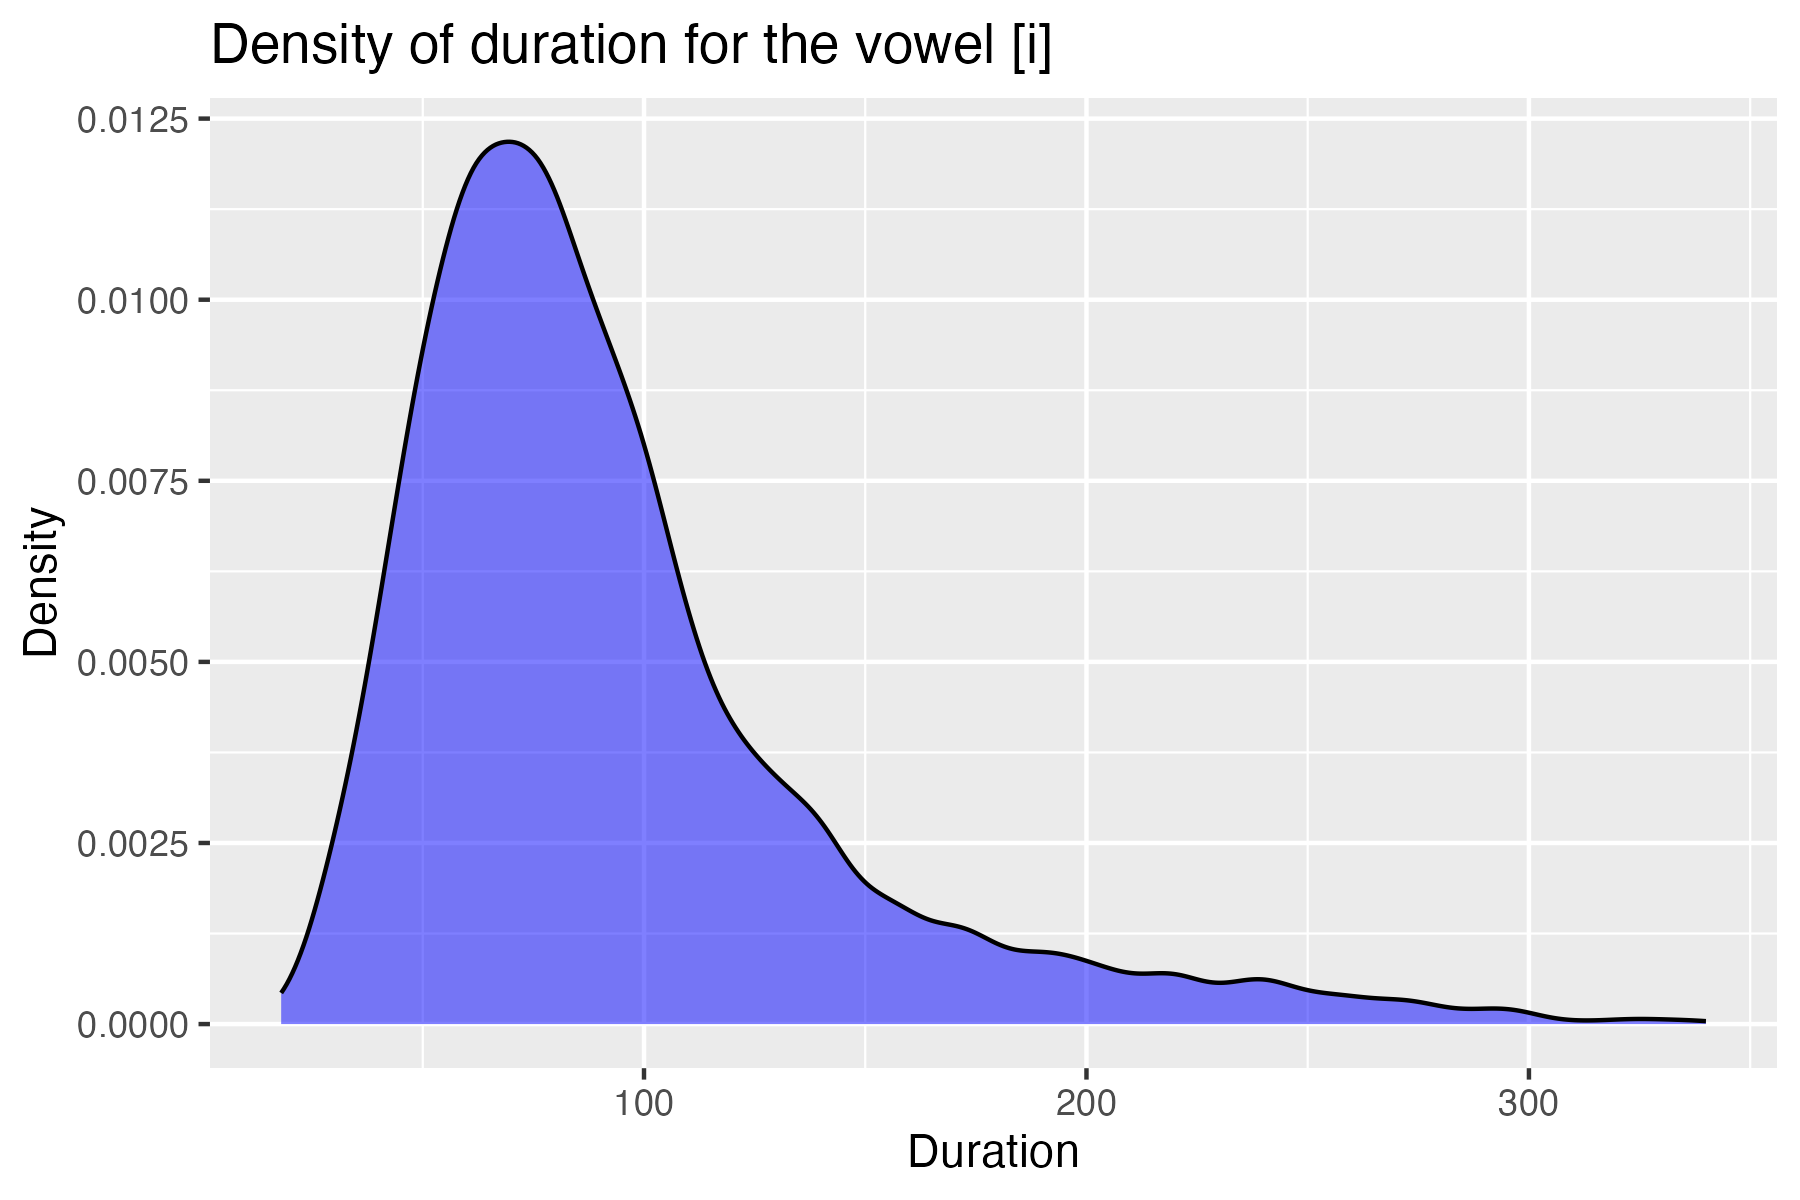
\includegraphics[]{problem1.png}
\end{center}

\begin{problem}{2}
Make a violin plot showing the distribution of durations for each vowel (you should see five blobs for five vowels). Use \texttt{draw\_quantiles} in \texttt{geom\_violin} to add the median to each blob. Which two vowels are the shortest on average? What do these two vowels have in common that distinguishes them from the other vowels?
\end{problem}

The shortest vowels on average are [i] and [u], which are also the only high ones.

\begin{center}
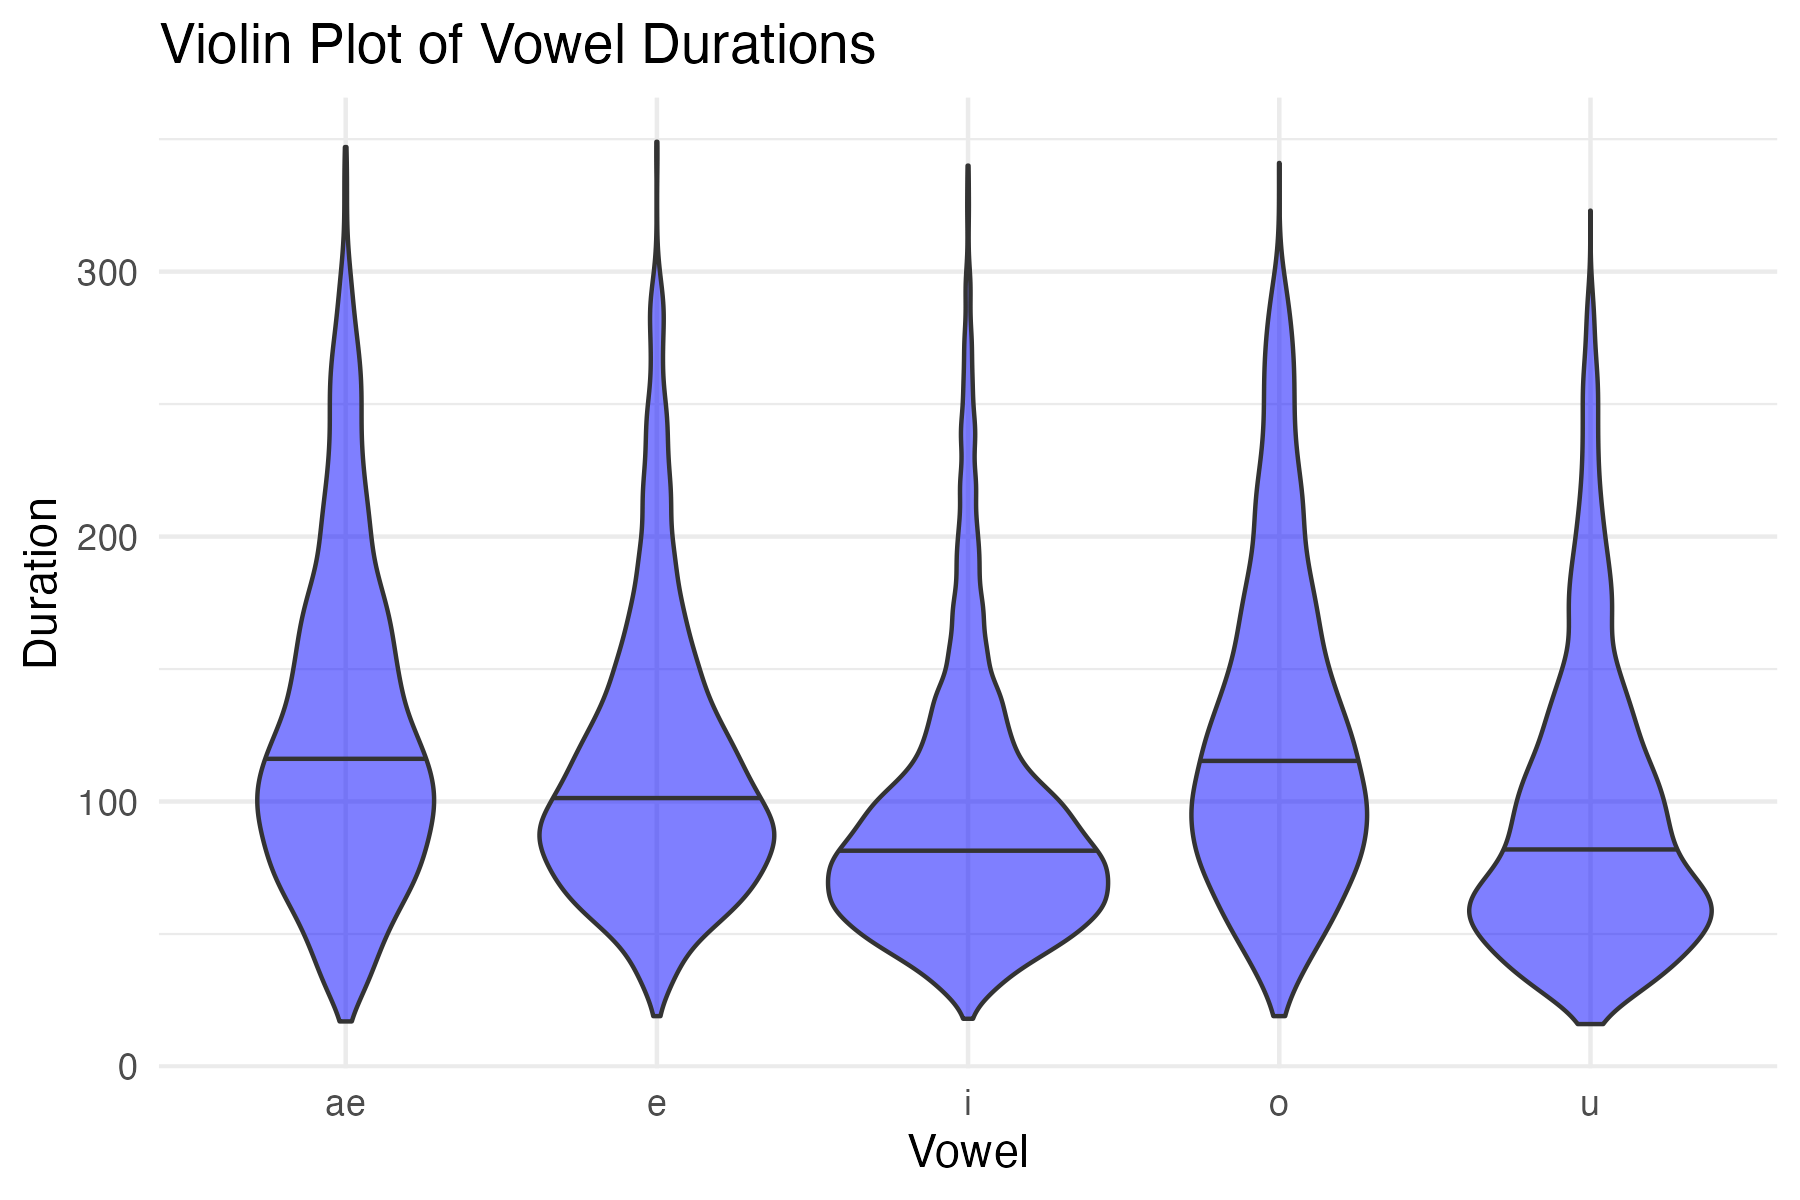
\includegraphics[]{problem2.png}
\end{center}

\begin{problem}{3}
Create a new data frame that only includes the vowels [i] and [e] for speaker 4. (Hint: to filter by condition 1 OR condition 2, use a bar \texttt{|} for OR.) What are the median durations of these two vowels for this speaker? Do the two vowels significantly differ? Perform a Wilcoxon test, and report W, p, and whether the test is significant.
\end{problem}

For speaker 4, the median durations of [e] and [i] are 85 ms and 53.5 ms respectively. A Wilcoxon test gives $W=30$ and $p=0.0162 < 0.05$ which means the test is significant. Thus, the vowels significantly differ for speaker 4.

\begin{problem}{4}
Returning to the original data frame with all speakers, make a scatter plot of vowel duration on the y-axis against word frequency (use the provided \texttt{freq} column) on the x-axis. Only include the vowel [i] in your plot. Add a smoother to the plot using \texttt{geom\_smooth}. Judging by the slope of the smoother, does duration tend to increase, decrease, or stay the same as frequency increases?
\end{problem}

The smoother has an overall negative slope, so the duration of [i] decreases as frequency increases generally.
\begin{center}
  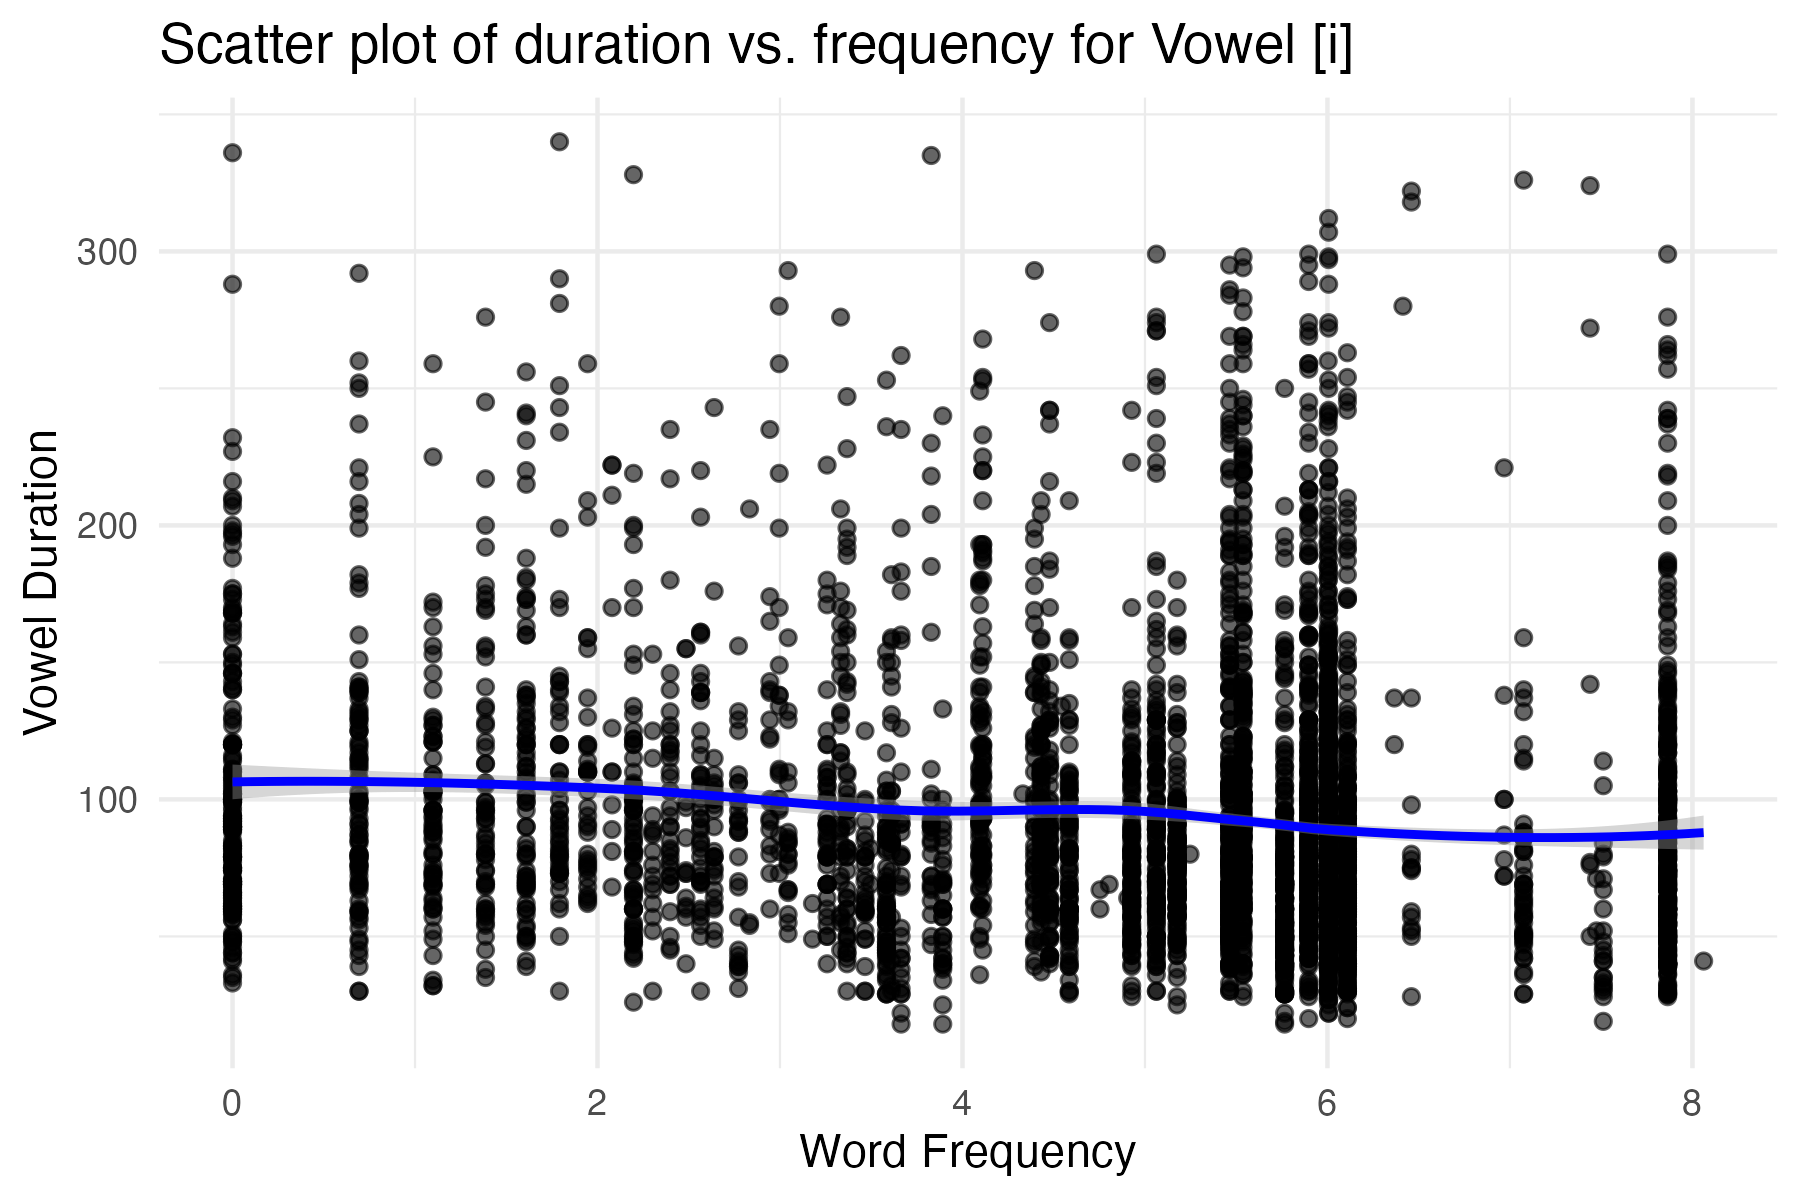
\includegraphics[]{problem4.png}
\end{center}

\begin{problem}{5}
Now switch to \texttt{words\_trimmed.txt} (which omits several columns so that the file is smaller). Use a regular expression (\texttt{str\_detect}) to determine how many word tokens contain a sequence of two or more nasals in a row in their Surface form. Take a nasal to be [mnN]. How many word tokens both begin and end with a nasal?
\end{problem}

The number of words with two or more nasals in a row in their surface form is 251, and the number of words that both begin and end with a nasal in their surface form is 3134.
% [1] "Percentage of time 't' is deleted in the word 'what': 64.6968534151957 %"
% [1] "Speaker with the highest deletion rate:"
% # A tibble: 1 × 2
%   Speaker deletion_rate
%     <int>         <dbl>
% 1      20           100
% [1] "Speaker with the lowest deletion rate:"
% # A tibble: 1 × 2
%   Speaker deletion_rate
%     <int>         <dbl>
% 1      38          29.0

\begin{problem}{6}
Speakers often delete the final t of a word such as \textit{what}, or turn it into a glottal stop. For simplicity, consider only the word \textit{what}, and count any alteration of the final t as deletion. In other words, \texttt{t\_deletes} (add this as a new column) is true whenever Surface does not end with t. Overall in the corpus, what percentage of the time does t delete in the word \textit{what}?
\end{problem}

The consonant `t' is deleted from ``what'' about $64.7\%$ of the time.

\begin{problem}{7}
Now do the same, except group the data by Speaker, and get each speaker’s mean rate of deletion. Which speaker deletes the most, and which the least? What are their rates of deletion?
\end{problem}

Speaker 20 deletes the most, at 100\% of the time, and speaker 38 deletes the least, at only 29\% of the time.

\begin{problem}{8}
Transmit Age and Gender into the previous question’s by-speaker summary, so that you can see that demographic information for each speaker. Make a box plot in which x is gender and y is the rate of deletion, faceted by age so that you can see four groups in total (2 × 2). Based on the plot, do women delete more or less often than men on average? Is there a clear interaction between age and gender? (In other words, is the effect of gender noticeably different between the two age groups? No need to be precise—we’re just asking if there’s an obvious difference or not.) No need to run any significance tests for this problem; you can just inspect the plot.
\end{problem}

As the plot shows, women delete more often than men on average, and the average deletion rate is more or less unaffected by age. As age increase, the variance in deletion rate increases.

\begin{center}
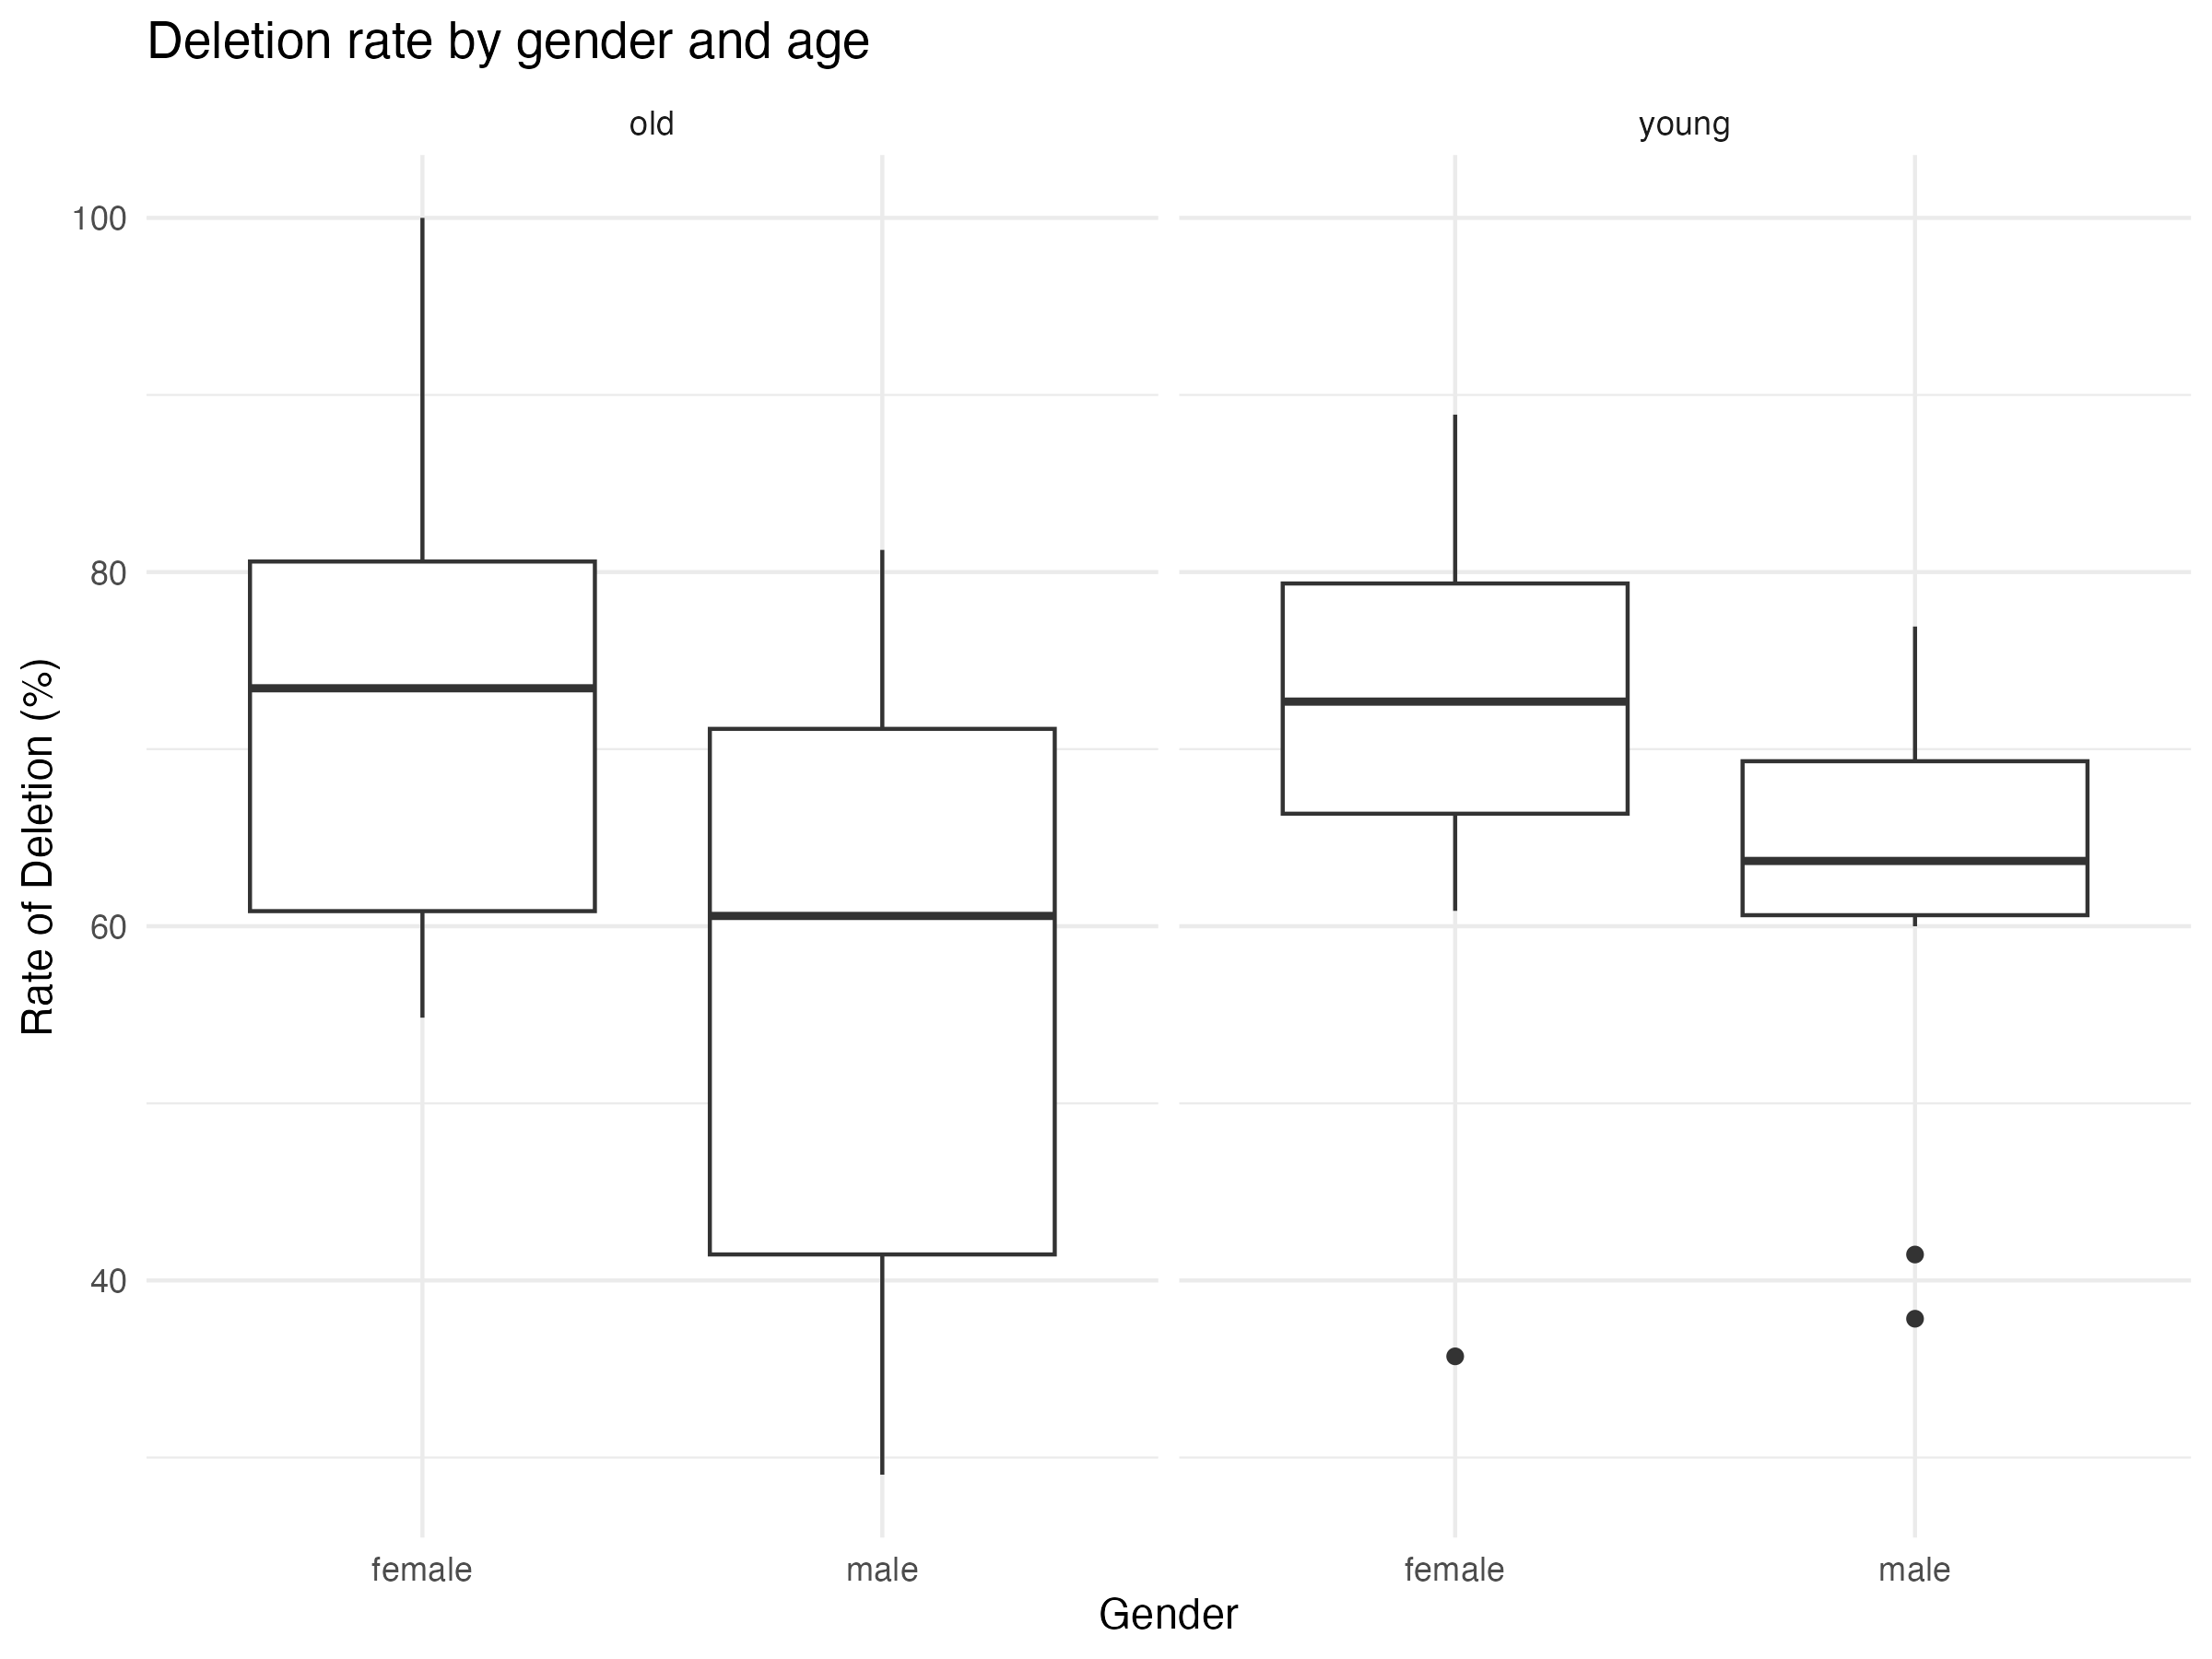
\includegraphics[]{problem8.png}
\end{center}

\end{document}
